\section{Сфера Римана}

Рассмотрим плоскость $XoY$ и касающуюся её в точке $O$ сферу
единичного диаметра. Точка $O$ -- южный полюс сферы, диаметрально
противоположный точке $P$ -- северному полюсу сферы. 

Возьмём комплексное число $Z$ на плоскости и пусть точка $M$ --
точка пересечения прямой $PZ$ и сферы.

Таким образом каждой точке плоскости можно сопоставить каждую точку 
сферы и, наоборот, каждой точке сферы (кроме $P$) можно сопоставить
каждую точку плоскости. Это соответствие называется стереографической
проекцией, а сфера -- \textbf{Сферой Римана}. 

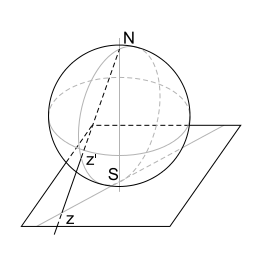
\includegraphics[scale=0.5]{riemannsphere}

Точке $P$ соответствует $z = \infty$ -- бесконечно удаленная точка.
Комплексную плоскость с бесконечно удаленной точкой $C$ называют
расширенную плоскостью и обозначают $\overline{\mathbb{C}}$.

